\documentclass[a4paper]{article}
\usepackage{graphics}

\usepackage[cover,dius]{nplreport}
\usepackage{hyperref}

\setlength{\topmargin}{0cm}
\setlength{\textwidth}{16cm}
\setlength{\textheight}{22cm}
\setlength{\oddsidemargin}{0cm}
\setlength{\evensidemargin}{0cm}
\setlength{\marginparwidth}{2cm}

\begin{document}

\newcommand{\vecc}[1]{\mbox{\boldmath $#1$}}
\renewcommand{\vec}[1]{\mathbf{#1}}
\renewcommand{\d}{\partial}
\renewcommand{\t}[1]{\mathrm{#1}}
\renewcommand{\div}{\nabla\cdot}

\newcommand{\grad}{\nabla}
\newcommand{\curl}{\nabla\times}
\newcommand{\eq}[1]{(\ref{#1})}
\newcommand{\f}[1]{Figure \ref{#1}}
\newcommand{\sect}[1]{Section \ref{#1}}
\newcommand{\dee}{\mathrm{d}}
\newcommand{\dd}[2]{\left(\frac{\d #1}{\d #2}\right)}
\newcommand{\ddd}[3]{\left(\frac{\d #1}{\d #2}\right)_{#3}}
\newcommand{\tensor}[1]{\underline{\underline{#1}}}
\newcommand{\emf}{\mathcal{E}}
\newcommand{\caf}{$\vec C,~\vec a,~\vec f$}
\newcommand{\zinc}{\textsc{Zinc}}
\newcommand{\zpp}{\textsc{Zpp}}
\newcommand{\uv}[1]{{\underline{#1}}}
\newcommand{\var}[1]{\texttt{#1}}

\NPLcentre{Materials Group}
\NPLapprovername{Markys Cain}
\NPLapproverjob{Knowledge leader for the Materials Team}
\NPLnumber{MAT}
\NPLyear{2016}

\title{ZINC 3.6 (Finite element code)\\Theory Manual} 
\NPLheader{ZINC 3.6 theory manual}

\author{John Blackburn} 
\date{February 2016}
\makecover
\maketitle

\begin{abstract}
This document describes the theory behind Zinc, a program for solving
arbitrary multiphysics systems using the finite element method.
\end{abstract}

\begin{prelude}\tableofcontents\end{prelude}

\section{Notation}
We use $(I,J,K)$ to represent the index of a node in a structured
mesh. The global node index is written as $\alpha$ or $\beta$ which
are a combination of the $I,J,K$ so that $\alpha=\alpha(I,J,K)$
etc. Independent variable numbers are written as $i$ or $k$ in the
range $1,2,..,N$ where $N$ is the number of variables. The index
within the FE vector is written as $p$ or $q$. These indices are a
combination of $\alpha$ or $\beta$ along with the independent variable
numbers $i$ or $k$ so that, eg, $p=p(\alpha,i)$. Spatial dimensions
are written as $j$ or $l$ and take values 1, 2 or 3. Variable $\ell$
is used to give local numbers of the nodes, $\ell=1,2,..8$. A
particular variable index is written as $s$, $s=1,2,...N$. There is no
implied summation over $s$.

Small vectors made of a list of variables are written in
\textbf{bold}. Eg, $\vec u=(u_1(\vec r),u_2(\vec r))$ (the position
vector is also written bold). Matrices corresponding to such vectors
are also written bold, eg, $\vec C$. The large FE vectors or matrices
are written underlined, eg, $\uv{u}$ is the vector of variable
values on each node. Correspoding matrices are written with a double
underline, eg, $\tensor{Q}$.

\section{Calculus of variations}
\label{theory}

Since most of the complexity of the method comes from the $C$ term, we
concentrate on this first then add the $a$ and $f$ terms in
\sect{adding}. We consider the static/harmonic case first and leave
the transient case untill \sect{trans}. We wish to solve the set of
equations
\begin{equation}
  (C_{ijkl}u_{k,l})_{,j}=0,~~~i=1,\ldots,N
\end{equation}
with natural boundary conditions
\begin{equation}
  n_j(C_{ijkl}u_{k,l})=0,~~~i=1,\ldots,N
\label{BC}
\end{equation}
We suggest this set of equations arises when we minimise the energy
function\footnote{Strictly this is an action function, the volume
integral of the system Lagrangian. It may or may not be the actual
energy of the system. We will use the term ``energy'' from now on with this caveat}
\begin{equation}
  U=\frac12 \int_V u_{i,j} C_{ijkl} u_{k,l}\, \dee V
  \label{energy}
\end{equation}
with respect to each $u_i$ function. To prove this write the change in
$U$ due to changing the function $u_s(\vec r)$ only, for a particular $s,~1\le s\le N$,
\begin{eqnarray*}
  U(u_s+\delta u_s)&=&\int\left[ \frac12 \sum_{jkl,k\ne s} (u_{s,j}+\delta u_{s,l}) C_{sjkl} u_{k,l}
+\frac12\sum_{ijl,i\ne s} u_{i,j} C_{ijsl} (u_{s,l}+\delta u_{s,l})\right.\\
&+&\frac12\left.\sum_{jl} (u_{s,j}+\delta u_{s,j})C_{sjsl}(u_{s,l}+\delta u_{s,l})\right]\,\dee V+\ldots
\end{eqnarray*}
The other terms are not affected by the change in $\delta
u_s$. Writing this out and discarding higher order tems in $\delta
u_s$, we can absorb the final two terms in the first two summations
(allowing $k$ or $i$ to equal $s$). This gives
\begin{equation}
  \delta U=U(u_s+\delta u_s)-U(u_s)=
\frac12\int \delta u_{s,j} C_{sjkl} u_{k,l}\, \dee V
+ \frac12\int u_{i,j} C_{ijsl} \delta u_{s,l}\, \dee V
\label{dU}
\end{equation}
There are two integrals but we require one. We must therefore insist
that 
\begin{equation}
  C_{ijsl}=C_{slij}
\label{Csym}
\end{equation}
which causes the two terms to be equal. The method we are currently
using -- minimising an Action function -- cannot solve problems where
this is not the case which implies the symmetry of the $C$ and, as we
will see later, the $a$ matrices. However, if the FE derivation was
done using a Galerkin formulation we could relax the restriction
\eq{Csym} and all the equations we derive from now on will still
apply. If the matrices are symmetrical, for a particular problem, then
it implies that problem can be written as an action minimisation
problem.

Let us consider the $j=1$ contribution to the
energy,
\begin{eqnarray}
 &{}& \int \int \int_1 \delta u_{s,1} C_{s1kl} u_{k,l}\, \dee x_1 \dee x_2 \dee x_3
=\int \int |\delta u_s (C_{s1kl} u_{k,l})|_{x_1^\t{min}}^{x_1^\t{max}}\dee x_2 \dee x_3 
\nonumber\\
&-&\int\int\int_1 \delta u_s (C_{s1kl} u_{k,l})_{,1} \,\dee x_1 \dee x_2 \dee x_3
\label{byparts}
\end{eqnarray}
For energy minimum, both terms on the RHS must be zero. The first term
is evaluated only on the $x_1$ max and min faces and the term which
must vanish is $C_{s1kl} u_{k,l}$ for each $s$ (implied sum over
$k,l$). We can write this by introducing the vector $\vec n$ which is
normal to the $x_1$ face, i.e., $\vec n=(1,0,0)$. We then have
$n_j C_{sjkl} u_{k,l}=0$ where the $\vec n$ simply ``selects'' the
$j=1$ term. The other terms in the $j$ summation of \eq{dU}, $j=2,3$ will
give $C_{s2kl} u_{k,l}$ vanishing on $x_2$ faces and $C_{s3kl}
u_{k,l}$ vanishing on $x_3$ faces. These expressions are also given by
$n_j C_{sjkl} u_{k,l}=0$ with $\vec n$ taking its right value on the
respective faces. Thus, we see that minimizing the energy implies the
boundary condition,
\begin{equation}
  n_j C_{ijkl} u_{k,l}=0,~~~i=1,2,3
\end{equation}
on each point on the boundary, where $\vec n$ is the unit normal at
that point. (We have proved this using integration by parts only for
cuboid shapes but hereby postulate it is true for all shapes). The second
term in \eq{byparts} gives a condition within the simulation volume. If we add
on the terms from $j=2$ and $j=3$ from \eq{dU}, these will simply add to the
integrand so we have
\begin{equation}
  \int \left[\delta u_s(C_{s1kl} u_{k,l})_{,1}
+\delta u_s(C_{s2kl} u_{k,l})_{,2}
+\delta u_s(C_{s3kl} u_{k,l})_{,3}\right]\,\dee V
\end{equation}
For this to be zero we must have
\begin{equation}
  (C_{ijkl} u_{k,l})_{,j}=0,~~~i=1,\ldots,N
\end{equation}
as required.

Now the $C$ array is, in general, $N\times d\times N\times d$ where
$d$ the number of dimensions. We can write it out as a matrix in the
following way, using $N=2$, $d=3$ as an example,
\begin{equation}
  \left[\begin{array}{ccc|ccc}
    C_{1111} & C_{1112} & C_{1113} & C_{1121} & C_{1122} & C_{1123}\\
    C_{1211} & C_{1212} & C_{1213} & C_{1221} & C_{1222} & C_{1223}\\
    C_{1311} & C_{1312} & C_{1313} & C_{1321} & C_{1322} & C_{1323}\\ \hline
    C_{2111} & C_{2112} & C_{2113} & C_{2121} & C_{2122} & C_{2123}\\
    C_{2211} & C_{2212} & C_{2213} & C_{2221} & C_{2222} & C_{2223}\\
    C_{2311} & C_{2312} & C_{2313} & C_{2321} & C_{2322} & C_{2323}
  \end{array}\right]
  \label{Cmat}
\end{equation}
If this matrix is symmetrical then \eq{Csym} is satisfied.  The significance
of this matrix appears next. We write out the set of dependent variables as
$\vec u$, the prepare $\grad\vec u$ as $(\grad u_1,~\grad u_2)$,
i.e. 6 components in this example. Multiplying the above matrix by
$\grad\vec u$ gives the 6-component vector
\begin{equation}
  \vec C\grad\vec u
\end{equation}
We write this as $(\vec a|\vec b)$ and define the divergence of this
as $(\div\vec a|\div\vec b)$ (ie divergence operates of groups of
$d$ numbers). This gives the required set of equations as
\begin{equation}
  \div (\vec C\grad\vec u)=0
\end{equation}
and the boundary conditions appear as
\begin{equation}
  \vec n\cdot\vec C\grad\vec u=0
\end{equation}
For example in the multiferroic case, $\vec u=(u_1,u_2,u_3,V,V_m)$
(see User Manual) and
\begin{equation}
  \grad\vec u=(u_{1,1},u_{1,2},u_{1,3}|u_{2,1},u_{2,2},u_{2,3}|u_{3,1},u_{3,2},u_{3,3}|
V_1,V_2,V_3|V_{m,1}, V_{m,2}, V_{m,3})
\end{equation}
Multiplying the C-matrix by this vector and comparing shows that
\begin{equation}
  \vec C\grad\vec u=(\sigma_{11},\sigma_{12},\sigma_{13},\sigma_{21},\sigma_{22},\sigma_{23},
\sigma_{31},\sigma_{32},\sigma_{33},D_1,D_2,D_3,B_1,B_2,B_3)
\end{equation}
Finally taking the div of this (in groups of 3 remember) gives
\begin{equation}
  \left[\begin{array}{c}
    \sigma_{11,1}+\sigma_{12,2}+\sigma_{13,3}\\
    \sigma_{21,1}+\sigma_{22,2}+\sigma_{23,3}\\
    \sigma_{31,1}+\sigma_{32,2}+\sigma_{33,3}\\
    D_{1,1}+D_{2,2}+D_{3,3}\\
    B_{1,1}+B_{2,2}+B_{3,3}
  \end{array}\right]
=0
\end{equation}
which is the required equations in the multiferroic case, while taking the dot
product with $\vec n$ (in batches of 3) gives
\begin{equation}
  \left[\begin{array}{c}
    n_1\sigma_{11}+n_2\sigma_{12}+n_3\sigma_{13}\\
    n_1\sigma_{21}+n_2\sigma_{22}+n_3\sigma_{23}\\
    n_1\sigma_{31}+n_2\sigma_{32}+n_3\sigma_{33}\\
    n_1 D_1+n_2 D_2+n_3 D_3\\
    n_1 B_1+n_2 B_2+n_3 B_3
  \end{array}\right]=0
\end{equation}
which are the required boundary conditions. It
is normally easier to prepare $\vec C$ in matrix form, the components
$C_{ijkl}$ can be deduced by comparing the matrix with a ``template'' like \eq{Cmat}.

\section{FE formulation}
\label{formulation}

\begin{figure}
  \scalebox{0.7}{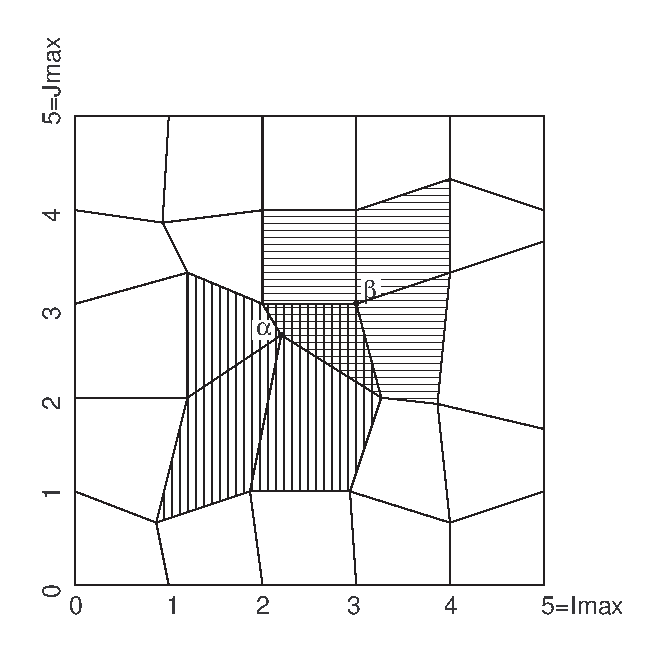
\includegraphics{fe}}
  \caption{Structured mesh (real mesh is 3-D) showing node numbering
  scheme and area of shape functions $N_\alpha$, $N_\beta$}
  \label{fe}
\end{figure}

This chapter uses material from \cite{afem}. We consider a 3-D
structured mesh made of hexahedrons as shown in \f{fe}. Mesh nodes
have are described by the coordinates $(I,J,K)$ and their positions in
space $(x,y,z)$. In reality the mesh will be distored to fit curved
surfaces etc, but the topology is always as shown. In the simulation,
an element is specified by quoting the coordinates of its 8
surrounding nodes.

We write the function $u_i$ as
\begin{equation}
  u_i(x,y,z)=\sum_\alpha u_{i\alpha} N_\alpha(x,y,z)
  \label{uxyz}
\end{equation}
where $\alpha(I,J,K)$ is a unique single number for each node (how we
generate $\alpha$ is unimportant but we must have a continuous sequence
of index numbers). $N_\alpha$ is a shape function with value 1 at
$\alpha$ and zero at any other node. It is non-zero only in the (maximum) 8
elements which surround the node $\alpha$. The shape function is
piecewise continuous, thus,
\begin{equation}
  N_\alpha=\left\{
  \begin{array}{c}
    N_\alpha^{(1)},~\t{in}~(1)\\
    N_\alpha^{(2)},~\t{in}~(2)\\
    N_\alpha^{(3)},~\t{in}~(3)\\
    :
  \end{array}\right.
\end{equation}
where 1,2,3,.. refer to the elements surrounding node $\alpha$. The
energy \eq{energy} can be written out as
\begin{eqnarray}
  U&=&\int \frac12 \sum_{ijkl}\left(\sum_\alpha u_{i\alpha}N_{\alpha,j}\right) 
C_{ijkl}(\vec r)
  \left(\sum_\alpha u_{k\alpha}N_{\alpha,l}\right)\,\dee V\\
&=&\frac12\int \sum_\alpha\sum_\beta\sum_{ijkl} u_{i\alpha}N_{\alpha,j}
C_{ijkl} u_{k\beta}N_{\beta,l}\,\dee V\\
&=&\frac12 \sum_{\alpha\beta}\sum_{ik} u_{i\alpha}u_{k\beta}
\int \sum_{jl} N_{\alpha,j} C_{ijkl} N_{\beta,l}\dee V\\
&=&\frac12\sum_{\alpha\beta}\sum_{ik} 
u_{i\alpha}Q_{i\alpha k\beta}u_{k\beta}
\end{eqnarray}
with
\begin{equation}
  Q_{i\alpha k\beta}=\int \left[\sum_{jl} N_{\alpha,j} C_{ijkl} N_{\beta,l}\right]\dee V
\end{equation}
The above integral is only non-zero in those elements which connect
$\alpha$ and $\beta$ so the integral can be written
\begin{equation}
  Q_{i\alpha k\beta}=\sum_{(e)}\int_{(e)} \left[\sum_{jl} 
N_{\alpha,j}^{(e)} C_{ijkl}^{(e)} N_{\beta,l}^{(e)}\right]\dee V=
\sum_{(e)}\sum_{jl}C_{ijkl}^{(e)}\int_{(e)} N_{\alpha,j}^{(e)}N_{\beta,l}^{(e)}
\,\dee V
\end{equation}
where $\sum_{(e)}$ refers to sum over all elements which connect
$\alpha,\beta$. The second expression might be quicker to calculate
numerically. Now, $\alpha$ and $\beta$ are global numbers, but we can
define corresponding \emph{local node numbers} $\ell_1$, $\ell_2$ from
1..8 for the element $(e)$ according to the scheme shown in \f{hexa}
(we will use $\ell$ for local index 1..8 while $l$ is a cartesian
direction 1..3). Then
%
\begin{figure}
  \scalebox{0.8}{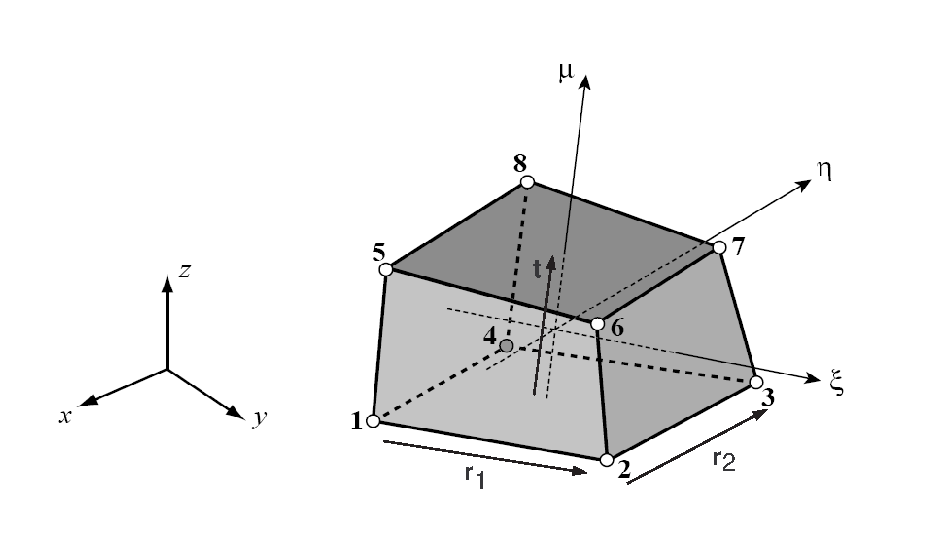
\includegraphics{hexa2}}
  \caption{Node numbering scheme for 8 node hexahedron. The nodes 1-4
  must be chosen so they are in the same face and numbered
  anti-clockwise viewed from the opposite face. This can be checked by
  calculating $\vec r_1\times\vec r_2$ and comparing with $\vec
  t$. Nodes 5-8 are opposite 1-4 as shown. After \cite{afem}}
  \label{hexa}
\end{figure}
%
\begin{equation}
  Q_{i\alpha k\beta}=\sum_{(e)}\int_{(e)} \left[\sum_{jl} 
N_{\ell_1,j}^{(e)} C_{ijkl}^{(e)} N_{\ell_2,l}^{(e)}\right]\dee V=
\sum_{(e)}\sum_{jl}C_{ijkl}^{(e)}\int_{(e)} N_{\ell_1,j}^{(e)}N_{\ell_2,l}^{(e)}
\,\dee V
\label{Qcomp}
\end{equation}
Now we define the shape function within the element according to local
coordinates $\xi$, $\eta$, $\mu$,
\begin{equation}
  N_\ell=\frac18(1+\xi\xi_\ell)(1+\eta\eta_\ell)(1+\mu\mu_\ell)
\end{equation}
where the corner $\xi_\ell$ etc are given by Table \ref{corner}.
\begin{table}
  \begin{tabular}{cccc}
    $\ell$ & $\xi_\ell$ & $\eta_\ell$ & $\mu_\ell$ \\ \hline
1 & $-1$ & $-1$ & $-1$ \\
2 & +1 & $-1$ & $-1$ \\
3 & +1 & +1 & $-1$ \\
4 & $-1$ & +1 & $-1$ \\
5 & $-1$ & $-1$ & +1 \\
6 & +1 & $-1$ & +1 \\
7 & +1 & +1 & +1 \\
8 & $-1$ & +1 & +1
  \end{tabular}
\caption{Local coordinate values for local node numbers, cf \f{hexa}}
\label{corner}
\end{table}
Given the shape function described in local coordinates we can
calculate the derivatives in \eq{Qcomp} as
\begin{eqnarray}
  \frac{\d N_\ell}{\d x}=\frac{\d N_\ell}{\d\xi}\frac{\d\xi}{\d x}
+\frac{\d N_\ell}{\d\eta}\frac{\d\eta}{\d x}
+\frac{\d N_\ell}{\d\mu}\frac{\d\mu}{\d x}\\
  \frac{\d N_\ell}{\d y}=\frac{\d N_\ell}{\d\xi}\frac{\d\xi}{\d y}
+\frac{\d N_\ell}{\d\eta}\frac{\d\eta}{\d y}
+\frac{\d N_\ell}{\d\mu}\frac{\d\mu}{\d y}\\
  \frac{\d N_\ell}{\d z}=\frac{\d N_\ell}{\d\xi}\frac{\d\xi}{\d z}
+\frac{\d N_\ell}{\d\eta}\frac{\d\eta}{\d z}
+\frac{\d N_\ell}{\d\mu}\frac{\d\mu}{\d z}
\end{eqnarray}
which can be written in matrix form
\begin{equation}
  \left[\begin{array}{c}
    {\d N_\ell}/{\d x}\\
    {\d N_\ell}/{\d y}\\
    {\d N_\ell}/{\d z}
  \end{array}\right]
=
\left[\begin{array}{ccc}
 {\d\xi}/{\d x} & {\d\eta}/{\d x} & {\d\mu}/{\d x} \\
 {\d\xi}/{\d y} & {\d\eta}/{\d y} & {\d\mu}/{\d y} \\
 {\d\xi}/{\d z} & {\d\eta}/{\d z} & {\d\mu}/{\d z} 
\end{array}\right]
\left[\begin{array}{c}
  {\d N_\ell}/{\d\xi}\\
  {\d N_\ell}/{\d\eta}\\
  {\d N_\ell}/{\d\mu}
\end{array}\right]
\label{dN}
\end{equation}
The above matrix is $\vec J_t^{-1}$, the inverse of the
Jacobian\footnote{Strictly the Jacobian is normally defined as the
transpose of $\vec J_t$ as presented here, hence the $t$ subscript to
indicate transpose}, $\vec J_t$
\begin{equation}
  \vec J_t=
  \left[  \begin{array}{ccc}
    \d x/\d\xi & \d y/\d\xi & \d z/\d\xi\\
    \d x/\d\eta & \d y/\d\eta & \d z/\d\eta\\
    \d x/\d\mu & \d y/\d\mu & \d z/\d\mu\\
  \end{array}\right]
\end{equation}
Now the functions $x$, $y$, $z$, can be expanded in terms of the
element shape functions
\begin{equation}
  x=\sum_{\ell=1}^8 x_\ell N_\ell,~~~
  y=\sum_{\ell=1}^8 y_\ell N_\ell,~~~
  z=\sum_{\ell=1}^8 z_\ell N_\ell
\label{xyz}
\end{equation}
Thus, using implicit summation, the Jacobian above can be written
\begin{equation}
  \vec J_t=
  \left[  \begin{array}{ccc}
    x_\ell\d N_\ell/\d\xi & y_\ell\d N_\ell/\d\xi & z_\ell\d N_\ell/\d\xi\\
    x_\ell\d N_\ell/\d\eta & y_\ell\d N_\ell/\d\eta & z_\ell\d N_\ell/\d\eta\\
    x_\ell\d N_\ell/\d\mu & y_\ell\d N_\ell/\d\mu & z_\ell\d N_\ell/\d\mu\\
  \end{array}\right]
\end{equation}
To perform the integral in \eq{Qcomp} we use
\begin{equation}
  \int_{(e)} f(x,y,z)\dee V=
\int_{-1}^1\int_{-1}^1\int_{-1}^1f(\xi,\eta,\mu)|\vec J_t|
\dee\xi\dee\eta\dee\mu
\end{equation}
(Note, we would normally use $|\vec J|$ above but the determinant of a
transpose is the same as that of the original matrix, so that $|\vec
J|=|\vec J_t|$). Thus we calculate $\vec J_t$ and use its determinant
in the integration and its inverse to deduce the derivatives wrt x, y,
z from \eq{dN}. The integrand above will be a polynomial and can be
evaluated exactly using Gaussian quadrature (In Gaussian quadrature we
need only evaluate $p$ points to integrate a $2p-1$ order polynomial)
\begin{equation}
\int_{-1}^1\int_{-1}^1\int_{-1}^1 ...\dee\xi\dee\eta\dee\mu=
\sum_{i=1}^{p_1}  \sum_{j=1}^{p_2}  \sum_{k=1}^{p_3}
f(\xi_i,\eta_j,\mu_k)|\vec J_t(\xi_i,\eta_j,\mu_k)|w_iw_jw_k
\end{equation}
where $\xi_i$ etc are special evaluation points between $-1$ and 1 and
$w_i$ are weights at these points. Some of these are listed next: 
\begin{equation}
  \begin{array}{rrrr}
    p & i & x_i & w_i \\ \hline
    1 & 1 & 0 & 2\\ \hline
    2 & 1 & -\sqrt{1/3} & 1\\
      & 2 & +\sqrt{1/3} & 1\\ \hline
    3 & 1 & 0 & 8/9\\
      & 2 & -\sqrt{3/5} & 5/9\\
      & 3 & +\sqrt{3/5} & 5/9
  \end{array}
\end{equation}
The integrand should be at most 5th order in any direction so we can
use $p_1=p_2=p_3=3$. Having developed $Q_{i\alpha j\beta}$ we can form
this into a matrix by defining the global coordinate
$p(i,\alpha)=1,2,3..$, $q(j,\beta)=1,2,3..$. Then
\begin{equation}
  U=\frac12 \sum_{pq} u_p Q_{pq} u_q=\frac12 \uv u^T \tensor Q \uv u
\end{equation}
Now, in simulation we wish to fix some of the $u_p$, that is some of
the variables in some of the nodes, so as to apply Dirichlet boundary
conditions. Thus, we minimise the energy only with respect to the
unknown variables in set $\mathcal{U}$.
\begin{equation}
  \frac{\d U}{\d u_p}=0,~~~p\in \mathcal U
\end{equation}
This gives the set of equations
\begin{equation}
  \sum_q \bar Q_{pq} u_q=0,~~~p \in\mathcal U
\end{equation}
where
\begin{equation}
  \bar Q_{pq}=\frac12(Q_{pq}+Q_{qp})
\end{equation}
In fact the matrix $Q$ will turn out to be symmetrical if $C$ is
symmetrical. If we want to solve unsymmetrical equations an
alternative Galerikin method can be used is not based on minimisation
of $\uv u^T\tensor Q\uv u$. In that case the equations are simply:
\begin{equation}
  \sum_q Q_{pq} u_q=0,~~~p \in\mathcal U
\end{equation}

These equations can be solved using the successive over relaxation
technique (SOR):
\begin{eqnarray}
  \bar Q_{pp} u_p^{(n+1)}=-\sum_{q\ne p} \bar Q_{pq} u_q^{(n)},~~p\in\mathcal U
  \label{iter1}\\
  u_p^{(n+1)}=u_p^{(n)},~~p\notin\mathcal U
\end{eqnarray}
 \zinc\ also includes a ``symmetrical SOR'' solver in which we set new
 values of $\vec u$ in terms only of old values, rather than making
 use of recent updates to vector components. This gives the iteration formula
\begin{eqnarray}
  \bar Q_{pp} u_p'=-\sum_{q\ne p} \bar Q_{pq} u_q^{(n)},~~p\in\mathcal U
  \label{iter}\\
  u_p'=u_p^{(n)},~~p\notin\mathcal U
\end{eqnarray}
and then
\begin{equation}
  u_p^{(n+1)}=\omega u_p'+(1-\omega) u_p^{(n)}~~\forall p
\end{equation}
where $\omega$ is a parameter between 0 and 1 and $(n)$ refers to the
iteration number with $u_p^{(0)}$ the initial guess. Note that $u$
components which are fixed, not in $\mathcal U$, are not altered
during the iteration and must be set at their right values to start
with. The variable values should be set to an initial condition, eg,
zero, at the beginning. In general the matrix $\bar \vec Q$ will be
enormous and must be stored in sparse format. In the computer we
store, \texttt{Qval(ip), iQ(ip), jQ(ip), ip=1,...,lenQ} where
\texttt{lenQ} is the number of non-zero components. \texttt{iQ} and
\texttt{jQ} are the row and column indices and \texttt{Qval} is the
matrix value. Even in sparse form the storage requirements can be
large especially for a multiphysics simulation with many variables. If
\texttt{nnod, nvar} are the total number of nodes and number of
dependent variables then \texttt{Qval} will contain about
\texttt{nnod*nvar$^2$*27} floating point numbers (the 27 is because
each node connects to 26 surrounding nodes giving non-zeros in the
matrix. There is also a self interaction).

Having solved for $\vec u$ we will want to evaluate the solution
$u_i(x,y,z)$. This is quite difficult as we do not know which element
the point $(x,y,z)$ is in. From \eq{uxyz} we have
\begin{equation}
  u_i(x,y,z)=\sum_{\ell=1}^8 u_{i\ell} N_\ell(\xi,\eta,\mu)
\end{equation}
where $\xi,\eta,\mu$ are the local coordinates in the given element
corresponding to $x,y,z$. These can be found by
numerically iterating \eq{xyz}, which are implicit, non-linear
equations for $\xi,\eta,\mu$. If $\xi,\eta,\mu$ are all in $[-1,1]$
then the point is in this element otherwise we must search other
elements until we find the point. The derivatives are given by
\begin{equation}
  u_{i,j}(x,y,z)=\sum_{\ell=1}^8 u_{i\ell} N_{\ell,j}(\xi,\eta,\mu)
\end{equation}
where the shape function derivatives can be calculated using
$J_t^{-1}$ as detailed above.

Finally, while total energy can be calculated from $\vec u^T\vec Q\vec
u/2$, we can calculate the energy in each element using
\begin{equation}
  U^{(e)}=\frac12\sum_{mno}\sum_{ijkl} 
u_{i,j} C^{(e)} u_{k,l} |\vec J_t|w_m w_n w_o
\label{elen}
\end{equation}
where $u_{i,j},~u_{k,l},~|\vec J_t|$ are all evaluated at
$(\xi_m,\eta_n,\mu_o)$ in the summation.

\section{Adding linear $a$ and $f$ terms to PDE}
\label{adding}

We now wish to generalise the PDE so that it includes the $a$ and $f$
terms. The PDE now reads,
\begin{eqnarray}
  -(C_{ijkl} u_{k,l})_{,j}+a_{ik} u_k=f_i\\
  -\div\vec C\grad\vec u +\vec a\vec u=\vec f
  \label{genPDE}
\end{eqnarray}
The BCs are unchanged. We do this by generalising the energy term to
\begin{equation}
  U=\int \left[\frac12 u_{i,j}C_{ijkl}u_{k,l}
+\frac12 u_i a_{ik} u_k-f_i u_i\right]\dee V
\end{equation}
Varying wrt $u_s$ gives
\begin{equation}
  \delta U=\int \left[-\delta u_s(C_{sjkl} u_{k,l})_{,j}
+\delta u_s a_{sk} u_k-\delta u_s f_s\right]\dee V
\label{delUadd}
\end{equation}
provided, in addition to \eq{Csym}, that,
\begin{equation}
  a_{ij}=a_{ji}
\end{equation}
Again, as noted previously, the condition of symmetry can be relaxed
and Zinc can cope with non-symmetrical situations. The restriction
comes about only because we have formulated the problem as an action
minimisation problem: the same equations could be derived with a
Galerikin method without the symmetry restriction. Setting
\eq{delUadd} to zero gives the required PDEs.

Labelling the new energy contribution $U_a$ and $U_f$ we obtain
\begin{eqnarray}
  U_a=\frac12\int\sum_{ik}\left(\sum_{\alpha}u_{i\alpha}N_\alpha\right)
a_{ik}\left(\sum_{\beta}u_{k\beta}N_\beta\right)\\
=\frac12\sum_{\alpha,\beta}\sum_{ik}u_{i\alpha}u_{k\beta}
\int N_\alpha a_{ik} N_\beta\,\dee V
=\frac12\sum_{\alpha,\beta}\sum_{ik}u_{i\alpha}u_{k\beta}P_{i\alpha k\beta}
\end{eqnarray}
where
\begin{equation}
  P_{i\alpha k\beta}=
\sum_{(e)}\int_{(e)} 
N_\alpha^{(e)}a_{ik}^{(e)}
N_\beta^{(e)}\,\dee V
=\sum_{(e)}a_{ik}^{(e)} \int_{(e)} N_\alpha^{(e)} N_\beta^{(e)}\,\dee V
\end{equation}
where the element sum is over elements connecting $\alpha$,
$\beta$. And
\begin{equation}
  U_f=-\sum_{i\alpha} u_{i\alpha} R_{i\alpha}
\end{equation}
with
\begin{equation}
  R_{i\alpha}=\sum_{(e)} f_i^{(e)}\int_{(e)}N_\alpha^{(e)}~\dee V
\end{equation}
where the element sum is over elements connected to $\alpha$.
Thus, the total energy is
\begin{eqnarray}
  U&=&\frac12\sum_{\alpha,\beta}\sum_{ik}u_{i\alpha}
(Q_{i\alpha k\beta}+P_{i\alpha k\beta})u_{k\beta}
-\sum_{i\alpha} u_{i\alpha}R_{i\alpha}\\
   &=&\frac12\uv u^T (\tensor Q+\tensor P)\uv u-\uv u^T\uv R
\end{eqnarray}
Equation \eq{iter} is generalised to
\begin{eqnarray}
  \overline{(Q_{pp}+P_{pp})} u_p'
=-\sum_{q\ne p} \overline{(Q_{pq}+P_{pq})} u_q^{(n)}+R_p,~~i\in\mathcal U
\end{eqnarray}
Finally, \eq{elen} is generalised to
\begin{equation}
  U^{(e)}=\sum_{mno}
\left[\frac12 u_{i,j}C_{ijkl}^{(e)}u_{k,l}
+\frac12 u_i a_{ik}^{(e)} u_k-f_i^{(e)} u_i\right]
|\vec J_t|w_m w_n w_o
\end{equation}
where $u_{i,j},~u_{k,l},~u_i,~u_k,~|\vec J_t|$ are all evaluated at
$(\xi_m,\eta_n,\mu_o)$ in the summation.

\section{Transient analysis}
\label{trans}

Consider advancing the solution vector $\uv u$ in the following scheme
\begin{equation}
  u_{\alpha,s}^{n+1}=u_{\alpha,s}^n-\frac{\delta t}{K_\alpha} 
  \frac{\delta U}{\delta u_{\alpha,s}}
\label{titer}
\end{equation}
where $n$ indicates the iteration number and $n=0$ is the initial
condition. This means that we alter the value of variable $s$ at the
node $\alpha$ leaving other nodal values constant. $\delta
u_{\alpha,s}$ is the amount we alter the nodal value by (note, $\delta
u_{\alpha,s}$ is not a function of space) and $\delta U$
is the consequent energy change. Thus, the amount we advance
$u_{\alpha,s}$ is proportional to the consequent rate of change of
energy. The factor $K_\alpha$ is given by
\begin{equation}
  K_\alpha=\int N_\alpha \dee V=\sum_{(e)}\int N_\alpha^{(e)} dV  
\end{equation}
i.e the integral over the shape functions surrounding the node in
question. In continuum terms we have perturbed the function $u_s(\vec
r)$ by adding a function $\delta u_s(\vec r)$ and $\delta U$ is the
energy difference before and after the perturbation:
\begin{equation}
  \delta U=U[u_s(\vec r)+\delta u_s(\vec r)]-U[u_s(\vec r)]
\end{equation}
$\delta u_s(\vec r)$ must be chosen so that it is equal to $\delta
u_{\alpha,s}$ at $\vec r=\vec r_\alpha$ and zero at other nodes. A
reasonable choice is
\begin{equation}
  \delta u_s(\vec r)=\delta u_{\alpha,s} N_\alpha(\vec r)
\end{equation}
It remains to specify $\delta u_{\alpha,s}$. We take it as
\begin{equation}
  \delta u_{\alpha,s}=\frac{u_{0s} V_0}{K_\alpha}  
\label{duas}
\end{equation}
Here, $u_{0s}$ is a constant in u-units and $V_0$ is a volume constant.
Thus, the amount we perturb the node value depends on the meshing
via $K_\alpha$. Thus, $\delta u_s(\vec r)$ becomes,
\begin{equation}
  \delta u_s(\vec r)=\frac{u_{0s}V_0 N_\alpha(\vec r)}{K_\alpha}
\to u_{0s}V_0\delta(\vec r-\vec r_\alpha)
\label{dus}
\end{equation}
The last statement indicates that as the meshing becomes fine, the
function tends towards a delta-function.

Now, from \sect{theory} (considering only the C-term) $\delta U$ is given by
\begin{equation}
  \delta U=-\int \left[\delta u_s(C_{s1kl} u_{k,l})_{,1}
    +\delta u_s(C_{s2kl} u_{k,l})_{,2}
    +\delta u_s(C_{s3kl} u_{k,l})_{,3}\right]\,\dee V
\end{equation}
Substituting from \eq{dus}, this becomes
\begin{equation}
  \delta U=-u_{0s} V_0[(C_{sjkl} u_{k,l})_{,j}]_\alpha
\label{dU2}
\end{equation}
Substituting \eq{dU2} and \eq{duas} in \eq{titer} gives
\begin{equation}
  u_{\alpha,s}^{n+1}=u_{\alpha,s}^n+\delta t [(C_{sjkl} u_{k,l})_{,j}]_\alpha
\end{equation}
In the limit $\delta t\to 0$ we obtain
\begin{equation}
  \frac{\d u_s}{\d t}=(C_{sjkl} u_{k,l})_{,j}
\end{equation}

The other energy terms work in a similar way and we obtain
\begin{equation}
  \frac{\d u_s}{\d t}=(C_{sjkl}u_{k,l})_{,j}-a_{sk}u_k+f_s,~~~s=1,2,..,N
\label{tpde}
\end{equation}
or, in matrix format,
\begin{equation}
  \frac{\d\vec u}{\d t}=\div \vec C\grad\vec u-\vec a\vec u+\vec f
\end{equation}
Now, in \eq{titer}
\begin{equation}
  U=\sum_q u_p (Q+P)_{pq} u_q-\sum_p R_p u_p
\end{equation}
Thus,
\begin{equation}
  \frac{\delta U}{\delta u_{\alpha,s}}=\frac{\d U}{\d u_{\alpha,s}}=
\sum_q \bar Q_{pq} u_{q}-R_p
\end{equation}
where we have contracted the indices $\alpha,s$ in the last equation.
The iteration scheme \eq{titer} becomes
\begin{equation}
  u_{\alpha,s}^{n+1}=u_{\alpha,s}^n-
  \frac{\delta t}{K_\alpha} \sum_q (\bar Q_{pq} u_{q}-R_p)
\end{equation}
Solving this iteration scheme will yield solutions that satisfy \eq{tpde}.

\section{Generalising the boundary conditions}

So far we have not included explicit boundary conditions in the
analysis. At Neumann boundaries, the boundary condition automatically
becomes:
\begin{eqnarray}
  n_jC_{ijkl}u_{k,l}=0
\end{eqnarray}
we wish to generalise this to
\begin{eqnarray}
  n_jC_{ijkl}u_{k,l}+q_{ik}u_k=g_i
\end{eqnarray}
The $q$ term would be, for example, an applied traction in elasticity
theory or a surface charge in electrostatic problems.

The generalised energy becomes
\begin{eqnarray}
  U=\int\left[\frac12 u_{i,j}C_{ijkl}u_{k,l}+\frac12 u_i a_{ik} u_k-f_i u_i\right]
~\dee V-\int u_i g_i~\dee S
+\frac 12 \int u_i q_{ik} u_k~\dee S
\end{eqnarray}
Following the analysis of \sect{theory}, we obtain
\begin{eqnarray}
  \delta U_s=\int \delta u_{s,j}C_{ijkl}u_{k,l}\dee V-\int \delta u_s g_s\dee S
+\int \delta u_s q_{sk}u_k\dee S+~\t{a,f~terms}
\end{eqnarray}
Using integration by parts and considering only the surface term we get
\begin{eqnarray}
  \delta U_s^{\t{surface}}=\int \delta u_s C_{sjkl}u_{k,l}n_j~\dee S
-\int \delta u_s g_s \dee S
+\int \delta u_s q_{sk}u_k\dee S
\end{eqnarray}
Insisting this be zero on the boundaries, this gives
\begin{eqnarray}
  n_jC_{ijkl}u_{k,l}+q_{ik}u_k=g_i
\end{eqnarray}
on the boundaries as required. In vector form, we can write this as
\begin{eqnarray}
  \vec n\cdot \vec C\grad\vec u=\vec g
\end{eqnarray}
In elastic problems, \sect{theory}, we saw that $\vec C\grad\vec u$ is
a vector of stresses, so that, in the elastic case, with $q=0$, we
would have
\begin{eqnarray}
  \tensor\sigma\cdot\vec n=\vec g
\end{eqnarray}
which implies that, in elastic problems, $\vec g$ is the applied
traction (a force per unit area) on the surface. In the case of
hydrostatic pressure, $p$, for example, $\vec g=-p\vec n$ where $\vec
n$ is the unit normal. In cases like this, the components of $\vec g$
will form a vector whose direction varies from point to point on the
surface. The variables $\vec g$ and $\vec q$ operate like \caf\ and
can be set to either constants or expressions (including zero where no
flux/force is applied). It is often helpful for the user to write such
expressions in terms of the unit normal (at the face centre) as well
as $x,y,z$ and the solved-for variables.

To implement this in FE, let us consider the $\vec q$ term first.
\begin{eqnarray}
  U_q=\frac 12 \int u_i q_{ik} u_k~\dee S
\end{eqnarray}
We introduce
\begin{eqnarray}
  u_i(x,y,z)=\sum_\alpha u_{i\alpha} N_\alpha
\end{eqnarray}
Here $u_{i\alpha}$ the value of variable $i$ stored on node $\alpha$,
a node on one of the surfaces of the system (each surface has its own
iterpolation system). $N_\alpha$ is a shape function which spans the
faces surrounding that node. It has value 1 on the node $\alpha$ and
zero on connecting nodes on the same surface. Note that $N_\alpha$
still exists in 3-D space since (a) the faces surrounding node
$\alpha$ are oriented in different directions and (b) quadrilateral
faces are not necessarily planar.

\begin{figure}
  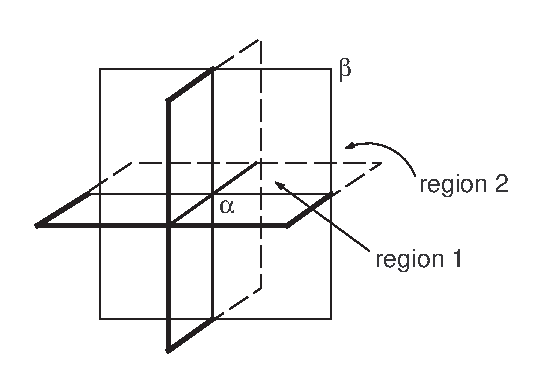
\includegraphics{surfaceint}
  \caption{Construction showing all faces connected to $\alpha$. In this case only one element face connects both $\alpha$ and $\beta$. \zinc\ will then check to see if a q-surface is defined between region 1 and region 2}
  \label{surfaceint}  
\end{figure}

Following the usual analysis, we obtain a contribution of
\begin{eqnarray}
U_q=\frac12\sum_{ik}\sum_{\alpha\beta}Q_{i\alpha k\beta} u_{i\alpha}u_{k\beta}\\
Q_{i\alpha k\beta}^q=\sum_{(f)}q_{ik}^{(f)}\int N_\alpha^{(f)}N_\beta^{(f)}\dee S
\end{eqnarray}
where the sum over faces includes faces connecting nodes $\alpha$ and
$\beta$. Since surfaces are defined as existing between spatial
regions, the program will check the region number of the element on
either side of the face and only apply the above contribution in the
case where the region number pair has an associated $q$ value (see \f{surfaceint}). The
face shape functions are
\begin{eqnarray}
  N_l(\xi,\eta)=\frac14(1+\xi\xi_l)(1+\eta\eta_l)
\end{eqnarray}
with
\begin{equation}
\begin{array}{ccc}
  l & \xi_l & \eta_l\\
1 & -1 & -1 \\
2 & +1 & -1 \\
3 & +1 & +1 \\
4 & -1 & +1
\end{array}  
\end{equation}
We can express the $x$ coordinate as
\begin{eqnarray}
  x=\sum_{l=1}^4 x_l N_l(\xi,\eta)
\end{eqnarray}
and similarly for the $y$ and $z$ coordinates. Then
\begin{eqnarray}
  \frac{\d\vec r}{\d\xi}=\left(\sum_l x_l\frac{\d N_l}{\d\xi},~
\sum_l y_l\frac{\d N_l}{\d\xi},~
\sum_l z_l\frac{\d N_l}{\d\xi}\right)\\
  \frac{\d\vec r}{\d\eta}=\left(\sum_l x_l\frac{\d N_l}{\d\eta},~
\sum_l y_l\frac{\d N_l}{\d\eta},~
\sum_l z_l\frac{\d N_l}{\d\eta}\right)\\
\end{eqnarray}
The surface integral becomes
\begin{eqnarray}
  \int N_\alpha^{(f)}N_\beta^{(f)}\dee S
=\int_{-1}^1\int_{-1}^1 N_\alpha^{(f)}N_\beta^{(f)}
\left|\frac{\d\vec r}{\d\xi}\times
\frac{\d\vec r}{\d\eta}\right|\dee\xi\dee\eta
\end{eqnarray}
Note that we need to take the magnitude of a vector meaning that the
integrand above will not be polynomial. However, it may be
sufficiently accurate to use Gaussian integration anyway. The local
numbers of element faces should be 1, 2, 3, 4 corresponding to a clockwise
or anticlockwise traversal around the face. The ``handedness'' does not
matter since we are computing a straightforward surface integral
($\int A\dee S$), not a flux integral ($\int \vec A\cdot\dee\vec S$).

Similarly, the $\vec g$ term contributes to the $R$ vector,
\begin{eqnarray}
U_g=-\sum_{i\alpha} u_{i\alpha} \int g_i N_\alpha \dee S=-\sum_{i\alpha} u_{i\alpha}R_{i\alpha}\\
R_{i\alpha}=\int g_i N_\alpha \dee S=\sum_{(f)} g_i^{(f)}\int N_\alpha^{(f)}\dee S
\end{eqnarray}
The sum over $f$ includes all faces connected to node $\alpha$: that
is all 12 faces shown in \f{surfaceint} (but only faces with a defined
\var{surface} command between corresponding regions will actually contribute). The integral is
\begin{eqnarray}
  \int N_\alpha^{(f)}\dee S
=\int_{-1}^1\int_{-1}^1 N_\alpha^{(f)}
\left|\frac{\d\vec r}{\d\xi}\times
\frac{\d\vec r}{\d\eta}\right|\dee\xi\dee\eta
\end{eqnarray}

\section{Testing if equations have been solved correctly}

\zinc\ solves the equations:
\begin{eqnarray}
  (\tensor P+\tensor Q)\uv u=\uv R
\end{eqnarray}
where the $C$, $a$ and $f$ matrices contribute to $\tensor P$,
$\tensor Q$ and $\uv R$ respectively. The residual is traditionally
defined as
\begin{eqnarray}
  (\tensor P+\tensor Q)\uv u-\uv R
\end{eqnarray}
However, in our case some of the degrees of freedom (components of $\uv
u$) are fixed, so we will gather these terms into the right hand
side. Considering components this gives
\begin{eqnarray}
  \sum_{j \in U}(P_{ij}+Q_{ij})u_j=R_i-\sum_{j \notin U}(P_{ij}+Q_{ij})u_j,
~~i \in U 
\end{eqnarray}
where $U$ is the set of unknown (not-fixed) degrees of freedom.  We
define the LHS vector $\uv l$ and RHS vector $\uv r$ as
\begin{eqnarray}
  l_i=\sum_{j \in U}(P_{ij}+Q_{ij})u_j~~i \in U\\
  r_i=R_i-\sum_{j \notin U}(P_{ij}+Q_{ij})u_j~~ i \in U\\
  l_i=r_i=0 ~~ i \notin U
\end{eqnarray}
We then define the residual as
\begin{eqnarray}
  \rho_i=l_i-r_i
\end{eqnarray}
Clearly if the equations have been solved we should have
\begin{eqnarray}
  \uv l=\uv r\\
  \uv \rho=\uv 0
\end{eqnarray}
To assess the accuracy of the solutions, \zinc\ outputs $|\uv \rho|$
and also
\begin{eqnarray}
  |\uv \rho|/|\uv l|
\end{eqnarray}
which is a dimensionless number less than 1. Here we take the usual
$\ell_2$ norm of the residual and LHS. Dividing by $|\uv l|$ gives a
number which does not scale with the number of degrees of
freedom. \zinc\ also outputs $|\uv l|$ and $|\uv r|$ directly -- these
numbers should be similar if the equations have been solved
correctly. Also, $|\uv \rho|$ should be much less than $|\uv l|$ or
$|\uv r|$.

\zinc\ also, optionally, outputs a graphical plot for of the residual
which can be viewed in \var{zmesh}. The user can see where the residual is
highest (rather than just seeing the total). If $\alpha=\alpha(I,J,K)$
is the unique index number of a node and $p=p(\alpha,i)$ is the unique
index number of a degree of freedom, then residual component $\rho_p$
is plotted on the $i$-th varible view of node $(I,J,K)$. Similarly the
$l_p$ and $r_p$ values can also be plotted on nodes under user
control. Of course degree of freedom $p$ is not uniquely determined by
equation $p$ but we can argue roughly that equation $p$ is the
``controlling equation'' for d.o.f. $p$.

\section{Alternative test based on finite differences}

\begin{figure}
  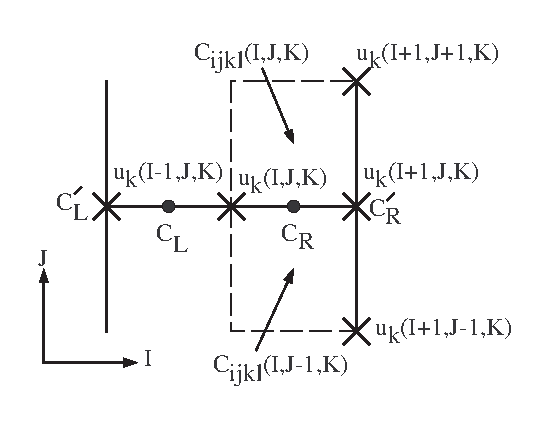
\includegraphics{fdchk}
  \caption{Geometry to calculate second derivatives using finite
    differences. The central line from $C_L'$ to $C_R'$ is used to
    calculate on axis second derivatives while the H-shape is used to
    calculated mixed derivatives}
  \label{fdchk}
\end{figure}

The formulation of residuals in the previous section is good for
checking that the linear equations derived from the FE formulation
have been solved correctly but does not check the accuracy of those
equations in the first place. To do that we can use a finite
difference (FD) technique which directly calculates second derivates
of the solution in order to check \eq{genPDE}: i.e. it does not make any
assumptions inherent in the finite element formulation given in
\sect{formulation}. However, \emph{this only works if all elements are
  cuboids}, it is up to the user to ensure this. If elements have been
distored the FD calculation will not give correct results. This FD-check
functionality has been put in \var{Zpp} as an optional post processing
step. The user can check any equation over any topological plane of
fixed index number. E.g. in a piezoelectric simulation, the user might
check the first equation (governing $u_x$) over the plane $i=15$. The
result is several surface plots with contributions from individual
variables shown separately. Thus in the piezoelectric example, with
$u=(u_x,u_y,u_z,V)$, \var{Zpp} will output contributions to the $C$
matrix from each of $(u_x,u_y,u_z,V)$. Contributions will similarly be
output for the $a$ and $f$ matrices. The sum total of all
contributions should be zero if the equations are satisfied. The user
will typically calculate the total and compare to one of the
components: the total should be much less than any component across
the scan area. The scan is done only over the interior of similation
area not the boundaries. Thus only the ``bulk'' PDEs are checked for
not the boundary conditions.

The differnential equaiton solved by \zinc\ is
\begin{eqnarray}
  -(C_{ijkl}u_{k,l})_{,j}+a_{ij}u_j=f_i
\label{fdeq}
\end{eqnarray}
Consider the structure shown in \f{fdchk} which is centred on the node
(I,J,K) which stores the solution $u_k$, with $k=1,\ldots,N$ where $N$
is the number of dependent variables. The figure is oriented in the
I-direction: we wish to consider first and second derivatives in this
direction and also mixed derivatives involving I and other directions
(direction J is shown in the figure giving an ``H'' shape). We can
define a first derivative on the left and right of the point (I,J,K):
\begin{eqnarray}
  \left(\frac{\d u_k}{\d x_l}\right)_L
  =\left\{
  \begin{array}{cc}
    (u_k(I,J,K)-u_k(I-1,J,K))/\Delta x_l & l=1\\
    (u_k(I,J,K)-u_k(I,J-1,K))/\Delta x_l & l=2\\
    (u_k(I,J,K)-u_k(I,J,K-1))/\Delta x_l & l=3
  \end{array}\right.\label{fdleft}\\
  \left(\frac{\d u_k}{\d x_l}\right)_R
  =\left\{
  \begin{array}{cc}
    (u_k(I+1,J,K)-u_k(I,J,K))/\Delta x_l & l=1\\
    (u_k(I,J+1,K)-u_k(I,J,K))/\Delta x_l & l=2\\
    (u_k(I,J,K+1)-u_k(I,J,K))/\Delta x_l & l=3
  \end{array}\right.\label{fdright}
\end{eqnarray}
These derivatives are conceptually defined at the dots shown in \f{fdchk} (or
equivalent points if $l=2,3$). According to \eq{fdeq} we need to couple these
derivatives to the $C_{ijkl}$ value and differentiate again. The
C-value is not uniquely defined at the dots, rather we shown take the
average of the C-values of elements shown in \f{fdchk} (the right hand
calculation is shown). We will call these values along $+l$ and $-l$, $C_R$ and $C_L$.

The on-axis second derivative along $l=j$ is given by
\begin{eqnarray}
  \frac{\d}{\d x_l}(C_{ijkl}\frac{\d u_k}{\d x_l})=
  \left[ C_R\left(\frac{\d u_k}{\d x_l}\right)_R-C_L\left(\frac{\d u_k}{\d x_l}\right)_L\right]/\Delta x_l
\end{eqnarray}
which is defined at $(I,J,K)$. For the mixed second derivatives with $j\ne l$ we have, for example, from \f{fdchk},
\begin{eqnarray}
  \frac{\d}{\d x_1}(C_{i1k2}\frac{\d u_k}{\d x_2})=
\frac{C_R'\frac{u_k(I+1,J+1,K)-u_k(I+1,J-1,K)}{2\Delta x_2}-C_L'\frac{u_k(I-1,J+1,K)-u_k(I-1,J-1,K)}{2\Delta x_2}}
{2\Delta x_1}
\end{eqnarray}
Here $C_R'$ and $C_L'$ are shown in \f{fdchk}: they are defined at
$(I+1,J,K)$ and $(I-1,J,K)$. In practice these must be taken as the
average C-value from the eight surrounding elements. The other mixed
derivatives can be calculated similarly: we need to go along the ``left''
and ``right'' directions indicated in \eq{fdleft}, \eq{fdright}, then branch out in a
perpendicular direction.

\begin{thebibliography}{9}
  \bibitem{fieldp} Field Precision Ltd, PO Box 13595, Albuquerque, New Mexico 87192 USA, www.fieldp.com
  \bibitem{meta} MetaMesh, Three-dimensional Conformal Mesh generator, Field Precision (2003).
  \bibitem{afem} ASEN 5367 -- Advanced Finite Element Methods, Carlos
A. Felippa, Aerospace Engineering Sciences, University of Colorado at
Boulder, www.colorado.edu, (2006), Chapter 18
\end{thebibliography}

\end{document}
